\section{Architekturdokumentation}\label{appendix:architekturdokumentation}

Die folgende Architekturdokumentation wurde parallel zum Projekt im Rahmen des Moduls Softwarearchitektur, -qualität und Testing (SAQT) an der Hochschule Luzern erarbeitet.

\subsection{Funktionale Anforderungen}\label{appendix:funktionale-anforderungen}
\subsubsection{Epics}
Die App soll folgende \textbf{Epics} erfüllen:
\begin{enumerate}
	\item \textbf{Bauanleitung (Guide):} Der Benutzer kann von einer gewählten Kugelbahn eine Augmented Reality Bauanleitung erhalten, um die Bahn physisch nachbauen/aufbauen zu können.
	\item \textbf{Baumodus (Builder):} Der Benutzer kann in Augmented Reality eine virtuelle Kugelbahn neu erstellen oder eine bestehende verändern, damit diese als Bauanleitung zur Verfügung stehen.
\end{enumerate}

\subsubsection{User Stories}\label{appendix:user-stories}

\begin{longtable}{l l p{13cm}}
	\hline
	\textbf{Nr.} & \textbf{Prio.} & \textbf{Beschreibung} \\
	\hline
	\textbf{1} & & \textbf{Allgemein} \\
	\hline
	1.1 & M &
		\begin{tabular}[t]{@{}p{13cm}@{}}
			Als Benutzer kann ich eine Fläche der realen Welt als Ebene für Augmented Reality auswählen, damit diese als Basis für die Anwendung verwendet wird. \\
			Akzeptanzkriterien:
			\begin{itemize}
				\item Von ARKit erkannte Flächen werden als rechteckige Flächen dargestellt.
				\item Durch antippen einer Fläche wird diese ausgewählt und alle anderen Flächen ausgeblendet und gelöscht.
				\item Die vertikale Position einer neu zu setzenden Kugelbahn orientiert sich an der ausgewählten Fläche, bzw. kommt darauf zu stehen.
			\end{itemize} \vspace*{-\baselineskip}
		\end{tabular} \\
	\hline
	1.2 & M &
		\begin{tabular}[t]{@{}p{13cm}@{}}
			Als Benutzer kann ich eine Kugelbahn auf der ausgewählten Ebene platzieren. \\
			Akzeptanzkriterien:
			\begin{itemize}
				\item Wenn eine Fläche ausgewählt ist, wird darauf eine Kugelbahn angezeigt.
				\item Die Kugelbahn befindet sich stets zentral im Kamerabild auf der Fläche.
				\item Durch Benutzereingabe, kann die Bahn an der aktuellen platziert werden.
			\end{itemize} \vspace*{-\baselineskip}
		\end{tabular} \\
	\hline
	1.3 & M & 
		\begin{tabular}[t]{@{}p{13cm}@{}}
			Als Benutzer kann ich die Kugelbahn auf einer Fläche ausrichten, damit sie wie gewünscht positioniert ist. \\
			Akzeptanzkriterien:
			\begin{itemize}
				\item Die Kugelbahn ist während des Platzierens stets zur Kamera ausgerichtet, sodass eine Drehung des Geräts auch die Rotation der Kugelbahn gegenüber der realen Welt verändert.
			\end{itemize} \vspace*{-\baselineskip}
		\end{tabular} \\
	\hline
	1.4 & M & 
		\begin{tabular}[t]{@{}p{13cm}@{}}
			Als Benutzer will ich erkennen in welchem Modus (Bauanleitung, Editor) ich mich befinde. \\
			Akzeptanzkriterien:
			\begin{itemize}
				\item Auf dem AR Bildschirm wird unmissverständlich angezeigt, welcher Modus aktiv ist.
			\end{itemize} \vspace*{-\baselineskip}
		\end{tabular} \\
	\hline
	1.5 & S & 
		\begin{tabular}[t]{@{}p{13cm}@{}}
			Als Benutzer kann ich die Position und Ausrichtung einer Kugelbahn korrigieren, damit sie mit der physischen Kugelbahn übereinstimmt. \\
			Akzeptanzkriterien:
			\begin{itemize}
				\item Die Position der Kugelbahn lässt sich über Bedienelemente in Richtung aller drei Achsen verschieben.
			\end{itemize} \vspace*{-\baselineskip}
		\end{tabular} \\
	\hline
	1.6 & K & 
		\begin{tabular}[t]{@{}p{13cm}@{}}
			Als Benutzer kann ich zwischen den Modi wechseln, damit ich die aktuelle Bahn im anderen Modus direkt weiterverwenden kann. \\
			Akzeptanzkriterien:
			\begin{itemize}
				\item Es besteht die Möglichkeit den aktiven Modus zu wechseln.
				\item Beim Wechsel bleibt die aktuelle Szene (Kugelbahn und Position) bestehen, die Fläche muss nicht neu erkannt und die Kugelbahn nicht neu gesetzt werden.
			\end{itemize} \vspace*{-\baselineskip}
		\end{tabular} \\
	\hline
	\textbf{2} & & \textbf{Guide} \\
	\hline
	2.1 & M & 
		\begin{tabular}[t]{@{}p{13cm}@{}}
			Als Benutzer kann ich eine gespeicherte Kugelbahn auswählen, um ihre Bauanleitung zu verwenden. \\
			Akzeptanzkriterien:
			\begin{itemize}
				\item Alle gespeicherten Kugelbahnen werden angezeigt und lassen sich auswählen.
				\item Die Kugelbahn, die für die Bauanleitung gesetzt wird entspricht der ausgewählten, gespeicherten Kugelbahn.
			\end{itemize} \vspace*{-\baselineskip}
		\end{tabular} \\
	\hline
	2.2 & M & 
		\begin{tabular}[t]{@{}p{13cm}@{}}
			Als Benutzer sehe ich, welches cuboro Element als nächstes physisch platziert werden soll. \\
			Akzeptanzkriterien:
			\begin{itemize}
				\item Das als nächstes zu bauende Element ist deutlich von den anderen Elementen hervorgehoben.
			\end{itemize} \vspace*{-\baselineskip}
		\end{tabular} \\
	\hline
	2.3 & M & 
		\begin{tabular}[t]{@{}p{13cm}@{}}
			Als Benutzer kann ich in der Bauanleitung einzelne Schritte vorwärts gehen, damit ich eine Bahn schrittweise aufbauen kann. \\
			Akzeptanzkriterien:
			\begin{itemize}
				\item Es gibt ein Bedienelement um den nächsten Schritt der Anleitung auszulösen.
			\end{itemize} \vspace*{-\baselineskip}
		\end{tabular} \\
	\hline
	2.4 & S & 
		\begin{tabular}[t]{@{}p{13cm}@{}}
			Als Benutzer kann ich in der Bauanleitung einzelne Elemente zurück gehen. \\
			Akzeptanzkriterien:
			\begin{itemize}
				\item Es gibt ein Bedienelement um zum vorhergehenden Schritt der Anleitung zurück zu gehen.
			\end{itemize} \vspace*{-\baselineskip}
		\end{tabular} \\
	\hline
	2.5 & K & 
		\begin{tabular}[t]{@{}p{13cm}@{}}
			Als Benutzer kann ich die Bauanleitung neu starten. \\
			Akzeptanzkriterien:
			\begin{itemize}
				\item Die Anleitung lässt sich direkt vom aktuellen Stand zurück auf den ersten Schritt zurücksetzen.
				\item Beim zurücksetzen bleibt die Position und Ausrichtung der Kugelbahn bestehen, es ist kein neu setzen notwendig.
			\end{itemize} \vspace*{-\baselineskip}
		\end{tabular} \\
	\hline
	\textbf{3} & & \textbf{Builder} \\
	\hline
	3.1 & M & 
		\begin{tabular}[t]{@{}p{13cm}@{}}
			Als Benutzer kann ich mindestens 4 verschiedene cuboro Elemente in der App verwenden, um eine Bahn zu erstellen. \\
			Akzeptanzkriterien:
			\begin{itemize}
				\item Bei der Auswahl des Elements stehen mindestens 4 unterschiedliche Typen zur Verfügung.
			\end{itemize} \vspace*{-\baselineskip}
		\end{tabular} \\
	\hline
	3.2 & M & 
		\begin{tabular}[t]{@{}p{13cm}@{}}
			Als Benutzer kann ich eine neue Kugelbahn erstellen und benennen. \\
			Akzeptanzkriterien:
			\begin{itemize}
				\item Bei der Wahl der Kugelbahn gibt es eine Option, eine neue Bahn zu erstellen.
				\item Beim Erstellen einer neuen Kugelbahn erhält der Benutzer die Möglichkeit einen Namen einzugeben.
				\item Die neu erstellte Kugelbahn erscheint in der Liste der Kugelbahnen mit ihrem Namen.
			\end{itemize} \vspace*{-\baselineskip}
		\end{tabular} \\
	\hline
	3.3 & M & 
		\begin{tabular}[t]{@{}p{13cm}@{}}
			Als Benutzer kann ich eine Kugelbahn auf dem Gerät speichern, damit ich sie später wiederverwenden kann. \\
			Akzeptanzkriterien:
			\begin{itemize}
				\item Die aktuelle Bahn kann durch den Benutzer gespeichert werden.
				\item Beim nächsten Abruf der Bahn erscheint diese im Zustand, in dem sie gespeichert wurde.
			\end{itemize} \vspace*{-\baselineskip}
		\end{tabular} \\
	\hline
	3.4 & M & 
		\begin{tabular}[t]{@{}p{13cm}@{}}
			Als Benutzer kann ich eine gespeicherte Kugelbahn bearbeiten. \\
			Akzeptanzkriterien:
			\begin{itemize}
				\item Der Benutzer kann eine gespeicherte Bahn auswählen.
				\item An der gewählten Bahn können Änderungen vorgenommen werden (Hinzufügen, Verändern oder Entfernen von Elementen).
			\end{itemize} \vspace*{-\baselineskip}
		\end{tabular} \\
	\hline
	3.5 & M & 
		\begin{tabular}[t]{@{}p{13cm}@{}}
			Als Benutzer sehe ich welche Positionen zur Wahl stehen, um ein Element hinzuzufügen. \\
			Akzeptanzkriterien:
			\begin{itemize}
				\item Valide Positionen für neue Elemente sind nach der Wahl des zu hinzufügenden Elements dargestellt.
				\item Valide Positionen sind nur solche, die physikalisch möglich sind (keine schwebende Elemente) und direkt an ein bestehendes Element anschliessen.
			\end{itemize} \vspace*{-\baselineskip}
		\end{tabular} \\
	\hline
	3.6 & M & 
		\begin{tabular}[t]{@{}p{13cm}@{}}
			Als Benutzer kann ich einer Kugelbahn ein neues Element an einer validen Position hinzufügen. \\
			Akzeptanzkriterien:
			\begin{itemize}
				\item Eine zur Wahl stehende Position kann ausgewählt werden, um an dieser Stelle das Element zu setzen.
				\item Das Platzieren abseits hervorgehobener Positionen ist nicht möglich.
			\end{itemize} \vspace*{-\baselineskip}
		\end{tabular} \\
	\hline
	3.7 & M & 
		\begin{tabular}[t]{@{}p{13cm}@{}}
			Als Benutzer kann ich ein die Ausrichtung (Rotation) eines Elements verändern. \\
			Akzeptanzkriterien:
			\begin{itemize}
				\item Ein Element kann ausgewählt werden und wird hervorgehoben.
				\item Durch Streichgesten kann das selektierte Element entlang einer der drei Achsen in Richtung der Geste um 90° gedreht werden.
			\end{itemize} \vspace*{-\baselineskip}
		\end{tabular} \\
	\hline
	3.8 & M & 
		\begin{tabular}[t]{@{}p{13cm}@{}}
			Als Benutzer kann ich ein Element von der Kugelbahn entfernen. \\
			Akzeptanzkriterien:
			\begin{itemize}
				\item Ein einzelnes Element kann von der Kugelbahn entfernt werden, solange die Kugelbahn zusammenhängend bleibt und physikalisch möglich ist (keine schwebende Elemente).
			\end{itemize} \vspace*{-\baselineskip}
		\end{tabular} \\
	\hline
	3.9 & S & 
		\begin{tabular}[t]{@{}p{13cm}@{}}
			Als Benutzer werde ich darauf aufmerksam gemacht, wenn Elemente nicht aneinander passen, damit ich am Schluss eine funktionierende/zusammenhängende Kugelbahn habe. \\
			Akzeptanzkriterien:
			\begin{itemize}
				\item Die App überprüft nach jeder Änderung der Kugelbahn, ob Rillen und Löcher der Elemente zusammenpassen und es einen durchgängigen Weg für die Kugel gibt.
				\item Elemente, die nicht zusammenpassen werden hervorgehoben oder markiert.
				\item Unpassende Elemente müssen nicht für das Funktionieren der App korrigiert werden, da es eine bewusste Entscheidung des Benutzers sein kann.
			\end{itemize} \vspace*{-\baselineskip}
		\end{tabular} \\
	\hline
\end{longtable}

\subsubsection{Zielhierarchie}
Abbildung \ref{fig:zielhierarchie-cockburn} zeigt einen Überblick über die Zielhierarchie der Anforderungen, zugeordnet nach den drei Farbstufen nach Cockburn.
\bild{0.9}{zielhierarchie-cockburn}{Zielhierarchie nach Cockburn}

\subsection{Nichtfunktionale Anforderungen}\label{appendix:nichtfunktionale-anforderungen}

\begin{longtable}{l l l p{10cm}}
	\hline
	\textbf{Nr.} & \textbf{Prio.} & \textbf{Typ} & \textbf{Beschreibung} \\
	\hline
	 & & Constraints & \\
	\hline
	01 & M & Technologie & Die App ist in Swift für iOS programmiert. \\
	02 & M & Technologie & Die App läuft auf aktuellen iPhones (ab iPhone 6s) mit iOS 11.3. \\
	03 & M & Technologie & Die App verwendet ARKit 1.5. \\
	04 & M & Geschäftlich & Die App zeigt die technologischen Möglichkeiten auf und muss keinen Business Value erzielen. \\
	\hline
	 & & Qualitäten & \\
	\hline
	05 & M & Laufzeit & Die App verwendet Farben, die auch für Personen mit Sehschwächen (z. B. Rot-Grün-Schwäche) erkenn- und unterscheidbar sind. \\ 
	06 & M & Laufzeit & Der Benutzer wird bei limitiertem Tracking Status über Massnahmen informiert. \\
	07 & M & Laufzeit & Beim Augmentieren von maximal 20 cuboro Elementen wird konstant mehr als 30 Frames pro Sekunde erreicht. \\
	08 & M & Laufzeit & Alle Daten der App werden nur lokal gespeichert (Offline). \\
	09 & M & Compilier-Zeit & Klassen- und Variablennamen im Code sind aussagekräftig. \\
	10 & M & Compilier-Zeit & Schlüsselstellen im Code sind gut kommentiert und verständlich aufgebaut. \\
	\hline
\end{longtable}

\subsection{Fachbegriffe}

\begin{itemize}
	\item \textbf{Element:} Ein einzelner cuboro Kugelbahnwürfel mit keinem (ganzer Würfel), einem oder mehreren Wegen für eine Kugel.
	\item \textbf{Kugelbahn:} Ein zusammenhängendes Konstrukt aus einzelnen Elementen, sodass eine Kugel einen durchgehenden Weg durch die Bahn hat.
	\item \textbf{Ebene:} Eine horizontale Fläche, die von ARKit als solche erkannt wird und als Untergrund für die Kugelbahn dient.
	\item \textbf{Bauanleitung:} Eine interaktive Anleitung, die den Benutzer schrittweise (Element um Element) durch den Aufbau einer Kugelbahn führt.
  \item \textbf{Tracking:} Der Vorgang, bei dem ARKit versucht Merkmale der realen Welt anhand Kamerabilder und Gerätesensoren zu verfolgen und anhand dessen die virtuellen Objekte ausrichtet.
  \item \textbf{Szene:} Die Lage des virtuellen Koordinatensystems in Referenz zur realen, physischen Welt. Dies umfasst die im virtuellen Raum platzierten Objekte (Kugelbahn).
\end{itemize}

\subsection{Systemkontext}

Das zu entwickelnde System (eine iOS App) interagiert mit dem Benutzer und mit den beiden Frameworks ARKit und SceneKit. Der Benutzer hält und bewegt das Gerät und über den Touchscreen mit der Benutzeroberfläche der App interagieren. Die App hält alle Daten lokal und hat keine Verbindung nach aussen zu irgendeinem anderen System oder Akteur.

\begin{figure}
  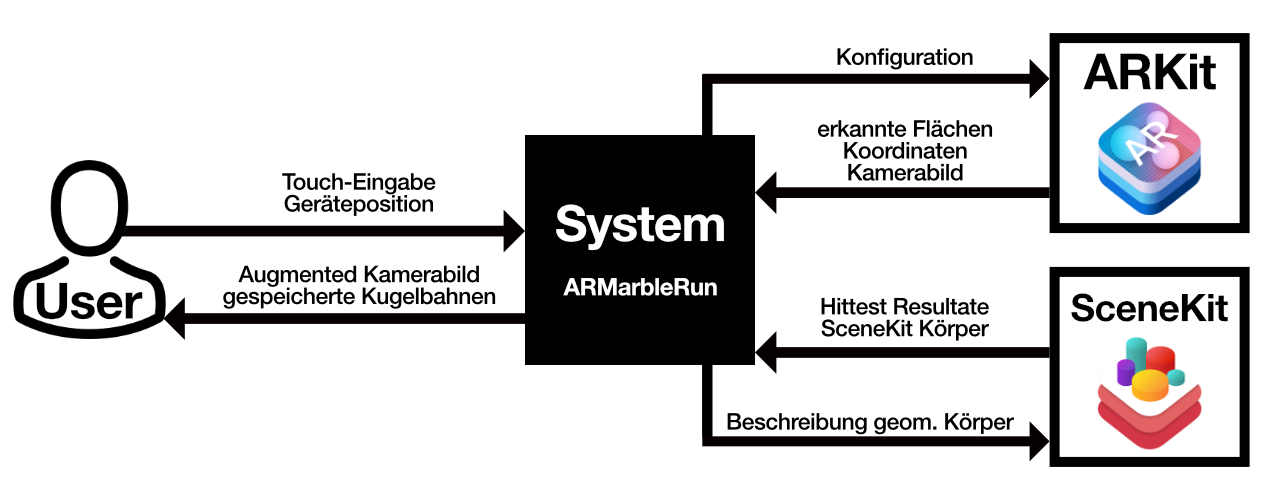
\includegraphics[width=\textwidth]{kontextdiagramm}
\end{figure}

\subsection{Systemvision}

Für Kugelbahnenthusiasten, cuboro Fans und solche die es noch werden wollen,
die ihre Kugelbahn mitnehmen wollen, planen wollen und nach Anleitung nachbauen wollen,
bietet unsere Kugelbahn App
mit Augmented Reality
eine komfortable, moderne und effiziente Methode seine Bahn zu planen oder zu bauen.
Anders als das offizielle cuboro Webkit,
ist die Kugelbahn mit der App mobil und man kann sie virtuell in einen realen Raum stellen.

\subsection{Architekturprinzipien}

Die zu entwickelnde Demo-App wird zu einem grossen Teil zum Selbstzweck erstellt.
Die App soll die ausgearbeiteten technologischen Möglichkeiten demonstrieren.
Der Code selber muss für an der entsprechenden Technik Interessierte hilfreich sein.
Dazu soll er informativ und verständlich sein.
Dies wird unter anderem mit \textbf{Selbstdokumentation} und der \textbf{Trennung von Verantwortlichkeiten} erreicht.
Die Trennung der Verantwortlichkeiten soll ausserdem dazu führen, dass einzelne Aufgaben/Teilprobleme gezielt studiert und wiederverwendet werden können.

\subsection{Taktiken}

Durch eine durchgehenden, starken Nutzung von Interfaces kann übersichtlich sichergestellt werden, welche Bestandteile der Software welche Aufgaben lösen. Die Interfaces sollen sprechene Methoden und Attributevariablen haben und wo notwendig mit Kommentaren ergänzt werden. Dieses Vorgehen hilft sowohl der Trennung von Verantwortlichkeiten und der Selbstdokumentation.

Weiter sollen Klassen möglichst klein und kohäsiv gehalten werden und zu zusammengehörigen Modulen gruppiert werden. Somit sollen interessante Stellen im Code rascher gefunden und verstanden werden. Das Vereinfacht die Wiederverwendung einzelner Module.

\subsection{Architekturstil}

Da die App monolithischen Charakter hat, also ohne Verbindungen nach Aussen und ohne Notwendigkeit zur Kommunikation mit verteilten Komponenten ist, fallen verteilte Stile (Client-Server, P2P usw.) weg.
Praktisch alle Abläufe in der App werden durch den Benutzer ausgelöst und führen zur Ausführung verschiedener Use Cases. Im Kern stehen die Kugelbahnen und deren Elemente.
Ein Stil nach dem Vorbild von Clean Architecture scheint daher passend zu sein: Events aus dem UI werden über Interfaces an verschiedene Interactor (Use Cases) weitergegeben, welche die Entities abrufen und bearbeiten.

Bei Recherchen stiessen wir auf die VIPER Architektur, welche versucht Clean Architecture spezifisch für iOS umzusetzen. Jeder Use Case ist ein VIPER Modul, das aus View, Interactor, Presenter, Entities und Wireframe (Router) besteht. Die Wireframes initialisieren ihr Modul und sind für das Aufrufen anderer Module verantwortlich. Der Interactor nutzt die globalen DataManager um Daten aufzurufen und für den Presenter bereitzustellen.

\begin{figure}
  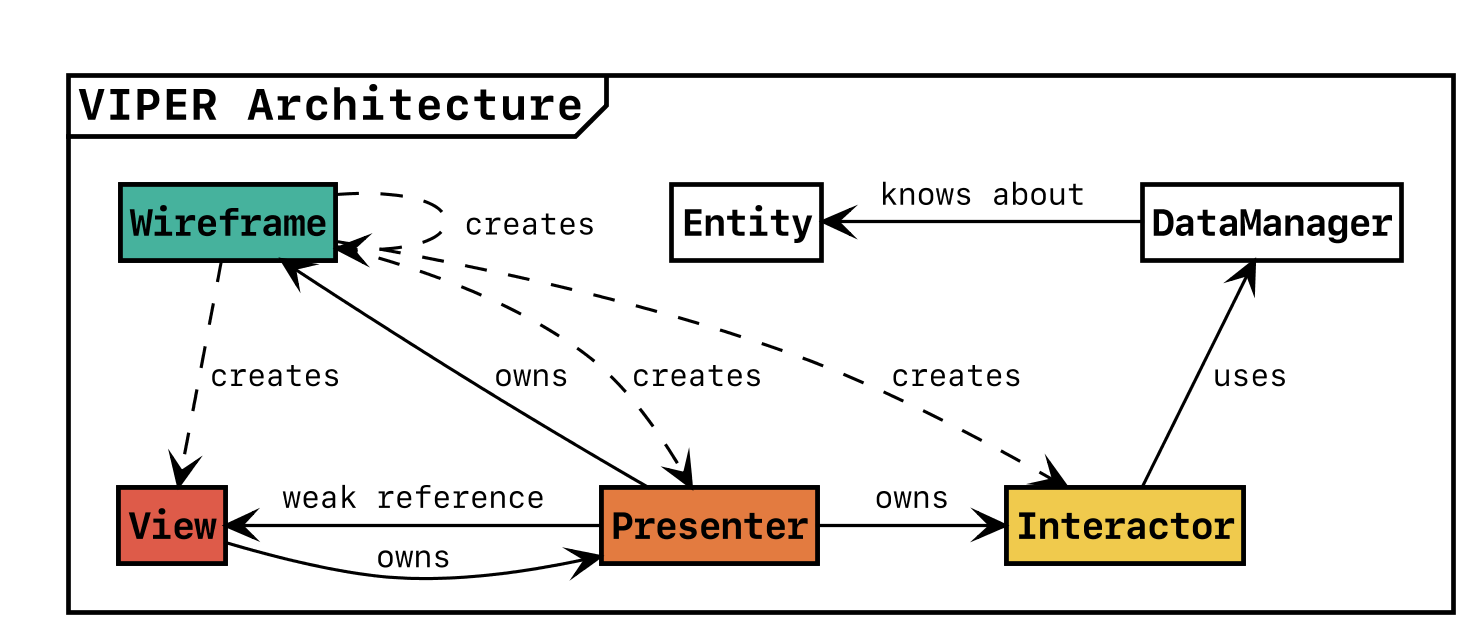
\includegraphics[width=0.8\textwidth]{viper-architecture}
\end{figure}

Die beiden wesentlichen Funktionen Bauanleitung (ARGuide) und Baumodus (AREditor) sind jeweils ein solches Modul. Sie teilen sich den DataManager, der Zugriff auf Kugelbahn- und Element-Entities hat. Daneben gibt es den Startbildschirm, bei dem der User den Modus wählen kann (SelectMode) und Listenansichten für Kugelbahnen (MarbleRunList) und Elemente (ElementList).

\begin{figure}
  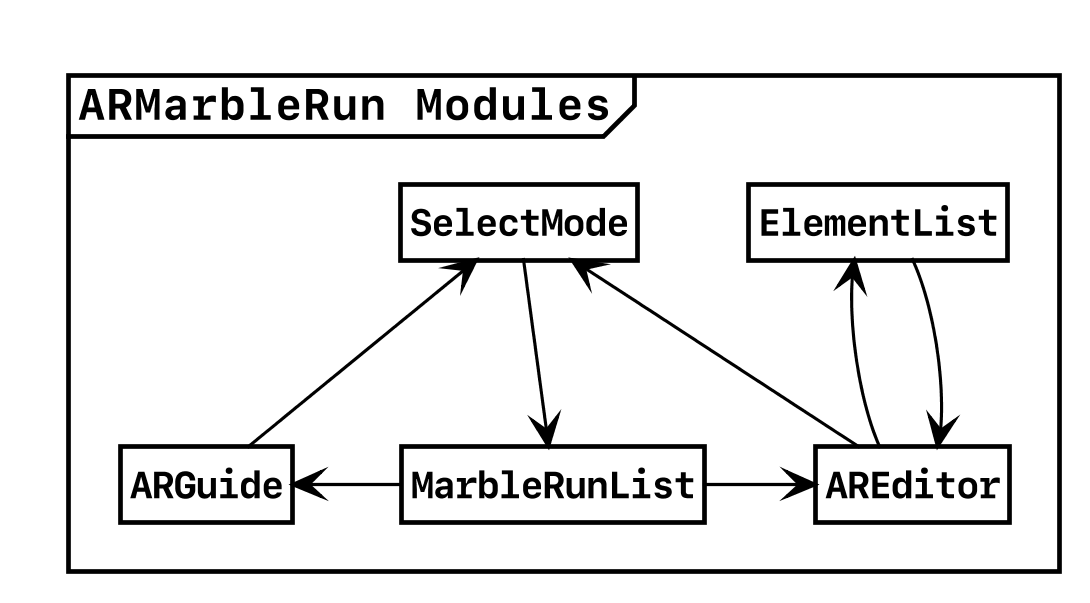
\includegraphics[width=0.5\textwidth]{viper-modules}
\end{figure}

\subsection{Systemsichten}

Alle Aktivitäten gehen von der View, bzw. vom Benutzer aus. Daher beginnt der folgende Fluss mit der View.

\begin{figure}
  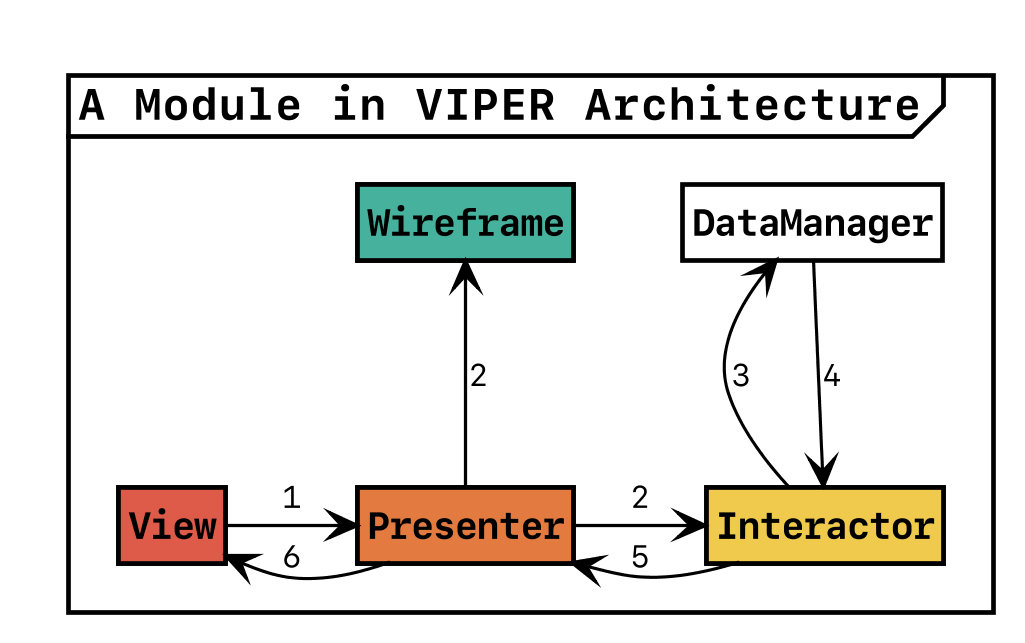
\includegraphics[width=0.5\textwidth]{viper-architecture-numbered}
\end{figure}

\begin{enumerate}
  \item Die View übergibt ein Event an den Presenter.
  \item Je nach Event wird entweder ein anderes Modul aufgerufen (via Wireframe) oder eine Anfrage nach Daten an den Interactor, der die Business Logik hat gerichtet.
  \item Der Interactor sendet einen Request nach Daten an den entsprechenden DataManager.
  \item Der DataManager gibt die gewünschten Entity Daten zurück.
  \item Der Interactor verarbeitet die Daten falls nötig und gibt sie an den Presenter weiter.
  \item Vom Presenter erhält die View nun Informationen, wie sie sich zu verändern hat.
\end{enumerate}

\subsection{Architekturentscheidungen}

Im folgenden zwei der wichtigsten Architekturentscheidungen:

\begin{table}
  \begin{tabular}{l p{13cm}}
    Issue         & 
      Der Benutzer soll zwischen den beiden Modi Baumodus und Bauanleitung wechseln können, ohne die virtuelle Kugelbahn neu im realen Raum zu platzieren. \\
    Alternatives  & 
      \begin{tabular}[t]{@{}p{13cm}@{}}
        Zwei Varianten:
        \begin{enumerate}
          \item Nur die relevanten UI Elemente (Buttons) ein-/ausblenden und eine Eventhandler Klasse verwenden, die ausgetauscht werden kann.
          \item Zwei getrenne Module machen, die sich die AR Szene mit den relevanten Informationen übergeben.
        \end{enumerate}
      \end{tabular} \vspace*{-\baselineskip}
      \\
    Outcome       & 2. Zwei getrennte Module. \\
    Rationale     &
      Eine saubere Trennung der unterschiedlichen Modi hilft der Nachvollziehbarkeit und Verständlichkeit des Codes und entkoppelt die Komponenten. Dies unterstützt ausserdem die Trennung der Verantwortlichkeiten und Erweiterbarkeit und bietet eine klarere Struktur. \\
  \end{tabular}
\end{table}

\begin{table}
  \begin{tabular}{l p{13cm}}
    Issue         &
      Die Elemente der aktuellen Kugelbahn müssen einerseits in der View als SceneKit Kindknoten der Kugelbahn zur Darstellung sein. Andererseits müssen sie in einem Konstrukt sein, das ihre logische Position und Nachbarn verwalten kann, um die Bauanleitung und Persistierung zu ermöglichen. \\
    Alternatives  &
      \begin{tabular}[t]{@{}p{13cm}@{}}
        Zwei Varianten:
        \begin{enumerate}
          \item Die SceneKit Knoten werden mit den notwendigen Informationen erweitert und zusammen mit logischen Koordinaten zusätzlich in einer Hashmap referenziert für die Business Logik.
          \item Die SceneKit Knoten werden rein auf ihre Funktion als UI Komponente reduziert und von zu persistierenden Entities getrennt.
        \end{enumerate}
      \end{tabular} \vspace*{-\baselineskip} \\
    Outcome       & 2. View und Entity trennen. \\
    Rationale     & 
      In Prototypen wurde Variante 1 versucht, dies führt jedoch zu starker Vermischung von Darstellung/View und der Business Logik. Die gewählte Variante stellt die Trennung von Verantwortlichkeiten sicher und erlaubt es zwischen der Darstellung von Persistierung von Kugelbahnen zu abstrahieren. Dadurch könnte das Datenformat geändert werden, ohne auch die Handhabung der 3D Element/Knoten komplett ändern zu müssen. \\
  \end{tabular}
\end{table}

